\setcounter{chapter}{21}
\chapter{Synthèse Organique (partie 2)}
\section{Représentation des molécules}

\subsection{Rappels}
revoir la nomenclature: savoir nommer une chaîne carbonée, identifier groupes caractéristiques et les familles organiques. 

\etiquette{Familles fonctionnelles}

\begin{center}
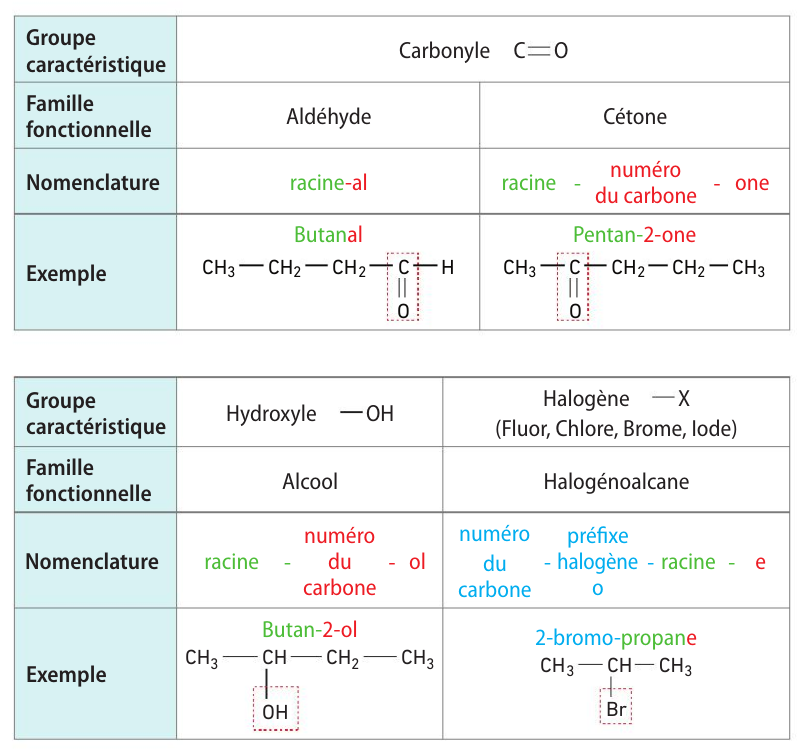
\includegraphics[scale=0.45]{figures/orga/fig_famille_1}\\
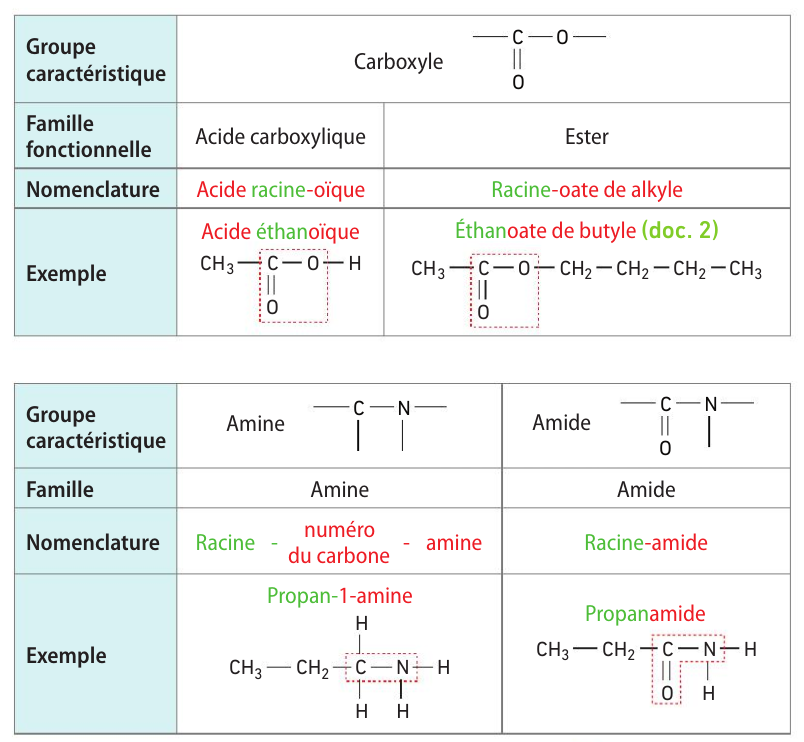
\includegraphics[scale=0.45]{figures/orga/fig_famille_2}
\end{center}

\section{L'isomérie de constitution}
\blocrouge{Définition}{
Deux espèces sont des isomères de constitution si \trou{elles ont la même formule brute mais des formules développées, semi-développées, topologiques différentes.}
}

Des isomères de constitution présentent souvent des propriétés physiques et chimiques \trou{différentes}.

\blocgris{Application}{
Trouver 2 isomères de l'espèce chimique ayant pour formule brute : $C_3H_6O_2$.
}

\section{Les polymères}
\blocrouge{Définition}{
Un polymère est une macromolécule, constituée d'un enchaînement répété d'un même motif, appelé \trou{monomère}, reliés les uns aux autres par des liaisons covalentes.
}

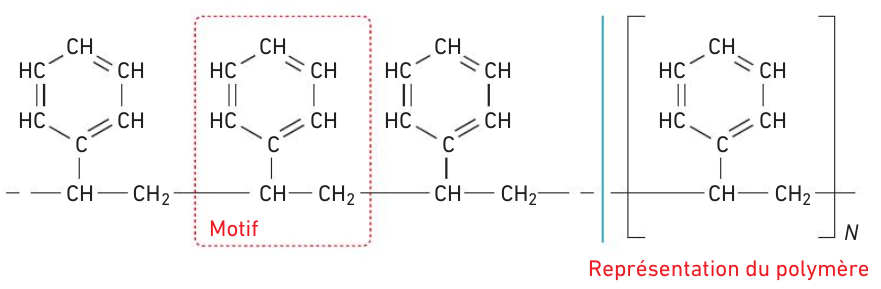
\includegraphics[scale=0.5]{figures/orga/fig_polymere}\\
On représente le polymère en écrivant le monomère entre crochets, avec le nombre de répétitions en indice.\\
Dans cette exemple, le monomère s'appelle le styrène, et le polymère le polystyrène.\\

\etiquette{Culture (au programme)} Les polymères peuvent être d'origine synthétique ou naturelle.\\
Par exemple, la cellulose que l'on trouve dans les mouchoirs en papier, ou le cis-polyisopropène que l'on trouve dans le latex sont d'origine naturelle.\\
Le polychlorure de vinyle ou PVC, que l'on trouve dans les revêtements de sol, les canalisations etc... est d'origine synthétique.



\section{La synthèse organique : optimisation de la vitesse et du rendement}
\subsection{Augmenter la vitesse d'une synthèse organique}

\begin{minipage}{0,7\linewidth}

Pour augmenter la vitesse de formation d'un produit, on peut :
\begin{itemize}
\item \trou{\textbf{Chauffer le milieu réactionnel} avec un montage à reflux pour éviter les pertes.}
\item \trou{\textbf{Augmenter la concentration} des réactifs en solution.}
\item \trou{ \textbf{Utiliser un catalyseur}. Le catalyseur est introduit en petite quantité dans le mélange réactionnel et il n'est pas consommé lors de la synthèse.}
\end{itemize}
Sur l'exemple ci-contre, on remarque que l'état final est le même, la quantité d'ester obtenue ne change pas, mais on atteint cet état final plus rapidement à 
$\SI{70}{\celsius}$ et encore plus rapidement si il y a un catalyseur.
\end{minipage}
\begin{minipage}{0,3\linewidth}

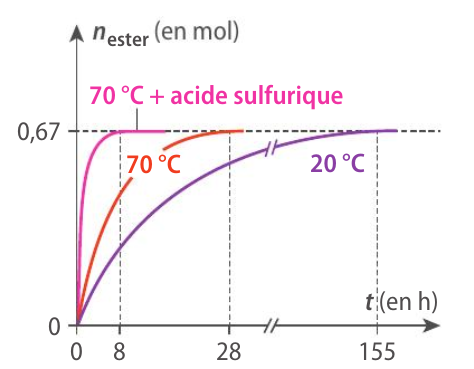
\includegraphics[scale=0.4]{figures/orga/fig_cinetique}
\end{minipage}
\subsection{Augmenter le rendement d'une synthèse organique}

\blocrouge{Définition}{
Le rendement d'une synthèse est \trou{le rapport entre la quantité de matière de produit  \trou{obtenu} et la quantité de matière théorique que l'on pourrait obtenir si la transformation chimique était \trou{totale} et qu'il n'y avait aucune perte.}
On le note : 
$$\eta=\dfrac{n_f}{n_{max}}=\dfrac{m_f}{m_{max}}$$ 
}

\subsection*{Constatations expérimentales}
On considère la réaction d'estérification, lors de laquelle un alcool réagit avec un acide pour donner un ester et de l'eau.\\
La réaction étudiée fait réagir l'éthanol et l'acide éthanoïque. L'ester obtenu est l'éthanoate d'éthyle.\\
La réaction s'écrit : 

$$CH_3CH_2-OH + CH_3-COOH\leftrightharpoons H-OH +CH_3COO-CH_2CH_3$$
$$\text{alcool} + \text{acide carboxylique}  \leftrightharpoons \text{eau}  + \text{ester}$$
On effecture 3 fois cette réaction pour des mélanges initiaux de réactifs différents. Les résultats obtenus sont:
\begin{center}
\begin{tabular}{l|cc||cc}
  & Etat Initial & (en mol) & Etat Final& (en mol)\\ \hline
  &$n_i(alcool)$ &$n_i(acide)$ &$n_f(ester)$&$n_f(eau)$\\
  \hline
 Cas n°1 &1,0&1,0&0,67&0,67 \\
 \hline
  Cas n 2 &1,0&5,0&0,946&0,946 \\
  \hline
  Cas n 3 &1,0&2,0&0,848&0,848 
\end{tabular}
\end{center}

\etiquette{Questions}
\begin{enumerate}
\item Quel est le réactif limitant dans chacun des cas ? Quelle est sa quantité de matière ?\\
\trou{Le réactif limitant est l'alcool dans chaque cas, et sa quantité de matière est égale à 1,0 mol.}
\item Calculer le rendement de la synthèse de l'ester dans chacun des cas.\\
\trou{Dans le cas 1, c'est 0,67\\
Dans le cas 2, c'est 0,94 et dans le cas 3, c'est 0,84}
\item Comparer l'évolution du rendement à l'évolution de la quantité de matière du réactif non limitant en fonction des différents cas. Que pouvez-vous conclure ?\\
\trou{On observe que plus la quantité de matière du réactif non limitant est importante, plus le rendement est élevé}
\item Cette observation est-elle en accord avec vos connaissances sur l'équilibre dynamique au niveau microscopique ?\\
\trou{En augmentant la quantité de matière de l'un des réactifs, la probabilité d'avoir des chocs efficaces entre les molécules de réactifs augmente, et donc $\tau_f$ augmente également}
\item En réfléchissant à l'équilibre dynamique au niveau microscopique, donner une autre idée qui permettrait d'augmenter le rendement de la synthèse.\\
\trou{En éliminant l'eau, cela évite que la transformation se fasse dans le sens indirect, et donc, cela augmente le rendement de la synthèse de l'ester}
\end{enumerate}

\blocrouge{Conclusion}{
Le rendement d'une synthèse augmente quand :
\vspace{0.3em}

\begin{itemize}
\item \trou{On introduit l'un des réactifs en excès}
\item \trou{On élimine du milieu réactionnel l'un des produits de la réaction.}
\end{itemize}
}



\etiquette{Exercices}
\begin{itemize}
	\item 10, 13 p 203
	\item 20, 21 p 204 
\end{itemize}

\etiquette{BAC}
\begin{itemize}
	\item \url{https://labolycee.org/optimisation-de-la-synthese-de-lethanoate-de-benzyle} : proche du cours
	\item \url{https://labolycee.org/larome-dananas} : Très complet
	\item \url{https://labolycee.org/le-nylon} : Polymère
\end{itemize}
 